\subsection{Le Réseaux des Neurones }
Pourquoi avons nous besoins du réseau des neurones? 
Supposons que nous avons un problème complexe de classification, la première approche serait d'utiliser la classification logistique avec un polynôme de plusieurs termes :

- cela conviendrait pour problème avec 1, ou 2 attribut.

- supposons maintenant que nous avons des  tuples avec plus de 1000 attributs ,

Ex: On veut prédire la chance d'une maison d'être vendu dans 6 mois  :
- Plusieurs facteurs entrent en jeu ,à peut près plus de 100 , on aura un polynôme avec les termes suivants (${x}_{1}^{2},{x}_{1}{x}_{2},{x}_{1}{x}_{3},{x}_{1}{x}_{4},...{x}_{1}{x}_{100}$),
on aura a peut près 5000 termes et ce nombre augmentera énormément si on choisi de considérer les 3 ème degré.
La régression logistique n'est pas vraiment approprié pour des problèmes de classification des données avec plusieurs attributs .

Par exemple dans le cas de la vision artificielle ou n peut aller de 2500 à 50000000  attributs.
On remarque bien qu'une simple régression logistique n'est pas approprié pour ce cas.

\subsubsection{Les Neurones et le cerveau\cite{NNBook}}

Une des motivations qui ont poussé les scientifique à créer le réseaux des neurones c'est celui de répliquer le fonctionnement du cerveau humain .
En effet le cerveaux humain dispose d'une capacité énorme d'apprentissage il s'apprend lui même comment apprendre et peut apprendre de n'importe quelle source des données,il  contient environ 100 milliards de neurones.
Voici à quoi ressemble à quoi ressemble un neurone dans le cerveau:
\begin{figure}[ht]
	\centering
	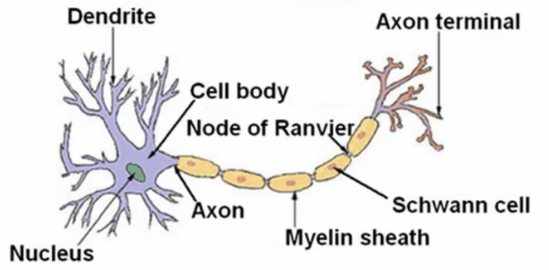
\includegraphics[width=0.5\textwidth]{fig/Neurone.png}
	\caption{Un Neurone Naturel}
	\label{fig:image9}
\end{figure}

Les neurones reçoivent les signaux (impulsions électriques) par des extensions très ramifiées de leur corps cellulaire (les dendrites) et envoient l'information par de longs prolongements (les axones). Les impulsions électriques sont régénérées pendant le parcours le long de l'axone. La durée de chaque impulsion est de l'ordre d'1 ms et son amplitude d'environ 100 mvolts.
Les contacts entre deux neurones, de l'axone à une dendrite, se font par l'intermédiaire des synapses. Lorsqu'un potentiel d'action atteint la terminaison d'un axone, des neuromédiateurs sont libérés et se lient à des récepteurs post-synaptiques présents sur les dendrites. L'effet peut être excitateur ou inhibiteur.
Chaque neurone intègre en permanence jusqu'à un millier de signaux synaptiques. Ces signaux n'opèrent pas de manière linéaire (effet de seuil).

\subsubsection{Représentation d'un Neurone Artificiel }
On pourrait définir un neurone  ou perceptrons comme étant une unité de traitement qui reçoit des données en entrée sous forme vectorielle et produit une sortie réelle , cette sortie est fonction des entrées et des poids de connexions.

Il se caractérise par :

- les signaux en entrée  ${x}_{1},{x}_{2},....,{x}_{n}$ ,

 il est toujours préférable d'ajouter le biais ${x}_{0}$ qui est égale à 1.,

- les coefficients synaptiques ou poids des connexions ${\theta}_{i0},{\theta}_{i1},....{\theta}_{in}$,

- Une Fonction d'activation ${h}_{\theta}(x)$,

- l'état interne d'activation $a={h}_{\theta}(x)$

\begin{figure}[ht]
	\centering
	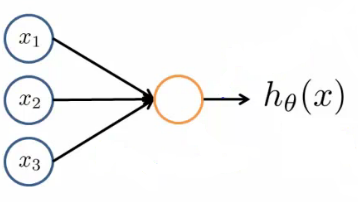
\includegraphics[width=0.5\textwidth]{fig/SimpleANN.png}
	\caption{un Perceptron  ou Unité de traitement}
	\label{fig:image10}
\end{figure}

D'une façon plus générale un  réseau des neurones est un ensemble de plusieurs neurones liés entre eux pour effectuer un calcul se compose :

- D'une couche d'entré ou activation layer 

- D'une couche de sortie ou output layer  

- D'une ou plusieurs couches intermédiaires ou hidden layers .

\begin{figure}[ht]
	\centering
	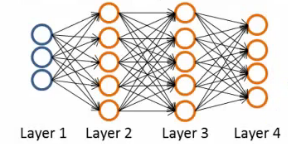
\includegraphics[width=0.5\textwidth]{fig/FullNeural.png}
	\caption{un réseau des neurones complets avec 2 hidden layers }
	\label{fig:image11}
\end{figure}

Chaque couche dispose des perceptrons ou unités d'activation.\\
On note :

 - ${a}_{i}^{j}$ : l'unité d'activation i de la couche j
 
 
 - ${\theta}^{l}$ : matrice des poids de connexions contrôlant le passage de la couche l à couche l+1.\\
 La matrice ${\theta}^{l}$ est constituée des termes ${\theta}_{ij}$ avec:
 
 - i l'indice de l'unité de la couche de destination
 
 - j l'indice de l'unité de la couche d'origine .\\
  Donc ${\theta}_{12}$ représente le poids de passage de l'unité 2 de la couche d'origine a l'unité 1 de la couche de destination.\\
 Regardons encore une fois l'image suivante :
\begin{figure}[ht]
 	\centering
 	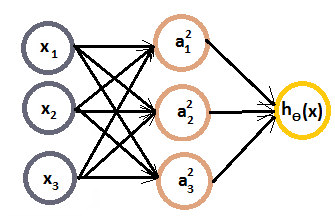
\includegraphics[width=0.5\textwidth]{fig/NeuralNtwork2.png}
 	\caption{Réseaux des neurones avec des unités d'activation }
 	\label{fig:image12}
\end{figure}\\
 Nous avons : \\
 ${a}_{1}^{(2) }= g({\theta}_{10}^{(1)}{x}_{0} + {\theta}_{11}^{(1)}{x}_{1} + {\theta}_{12}^{(1)}{x}_{2} + {\theta}_{13}^{(1)}{x}_{3})$ \\
 ${a}_{2}^{(2) }= g({\theta}_{20}^{(1)}{x}_{0} + {\theta}_{21}^{(1)}{x}_{1} + {\theta}_{22}^{(1)}{x}_{2} + {\theta}_{23}^{(1)}{x}_{3})$ \\
 ${a}_{3}^{(2) }= g({\theta}_{30}^{(1)}{x}_{0} + {\theta}_{31}^{(1)}{x}_{1} + {\theta}_{32}^{(1)}{x}_{2} + {\theta}_{33}^{(1)}{x}_{3})$ \\
 ${h}_{\theta}(x) ={a}_{1}^{(3) }= g({\theta}_{10}^{(2)}{a}_{0}^{(2)} + {\theta}_{11}^{(2)}{a}_{1}^{(2)} + {\theta}_{12}^{(2)}{a}_{2}^{(2)} + {\theta}_{13}^{(2)}{a}_{3}^{(2)})$ \\
 
 Chaque unité d'activation de la couche l+1 est obtenue en appliquant la fonction g (une sigmoïde ) aux à la combinaison linéaire des unités de la couche précédente avec les éléments de la matrice ${\theta}^{l}$. \\
 \subsubsection{Apprentissage par Réseau des neurones }
 Le réseau des neurones est un des plus puissant algorithme d'apprentissage ,
 il cherche à trouver les paramètres du modèle d'apprentissage uniquement à partir de l'ensemble d'apprentissage .\\
 Voici notre configuration :
 
 - Notre ensemble d'apprentissage est : {$({x}^{1},{y}^{1}),({x}^{2},{y}^{2}),({x}^{3},{y}^{3}),....({x}^{n},{y}^{m})$}
 
 - L nombre des couche de notre réseau . Pour notre cas L=4
 
 -${s}_{l}$ nombre des unités dans la couche l\\
 Donc en se référant à la \figurename{ 11} On remarque que :
 
 - L= 4
 
 - ${s}_{1} = 3$
 
 - ${s}_{2} = 5$
 
 - ${s}_{3} = 5$
 
 - ${s}_{4} = 4$
 
 Avec le réseaux des neurones on peut faire aussi bien des classification binaires que des classifications avec plusieurs classe.\\
 Pour la classification binaire la couche de sortie ne comprend qu'une seule unité k = 1 avec k le nombre des unités de la couche  de sortie.\\
 Pour une classification multi-classe k prend des valeurs supérieurs à 3,\\ la sortie  $y \in {\LARGE R}^{K} $  Pour 3 classes ${y}^{1} = [1,0,0]$ , ${y}^{2} = [0,1,0]$ , ${y}^{3} = [0,0,1]$; 
 \subsubsection{Fonction Cout}
 
 Rappelons que pour la régression logistique la fonction cout régularisée est la suivante :
 
\begin{center}
 	$J\left({\theta }\right)=\frac{1}{2m}[\sum _{i=1}^{m}-{y}^{(i)}\log [{h}_{\theta}\left({x}^{(i)}\right)] -(1-{y}^{(i)})\log [1-{h}_{\theta}\left({x}^{(i)}\right)] + {\lambda} \sum _{j=1}^{n}{{\theta}_{j}^{2}}]$
\end{center} 
 Pour le réseau des neurones la  fonction cout n'est que la généralisation de celui de la régression logistique mais au lieu d'une sortie nous avons K sorties .
 
 ${h}_{\theta}\left(x\right) \in {\LARGE R}^{k} $  et 
 $({h}_{\theta}\left(x\right))_{k} = {k}^{eme} $  sortie 
 
 
  	$J\left({\theta }\right)=\frac{1}{2m}[\sum _{i=1}^{m}\sum _{k=1}^{K}-{y}_{k}^{(i)}\log [({h}_{\theta}\left({x}^{(i)}\right))_{k}] -(1-{y}_{k}^{(i)})\log [1-({h}_{\theta}\left({x}^{(i)}\right))_{k}] + {\lambda} \sum _{l=1}^{L-1}\sum _{i=1}^{{s}_{l}}\sum _{j=1}^{{s}_{l+1}}{({\theta}_{ji}^{(l)})^{2}}]$ \\

Une fois la fonction cout connu le reste du travail consiste à entrainer notre réseau , donc de  trouver :

- la valeur des unités d'activation ${a}^{l}$ pour chaque couche 

- Ainsi que celles de ${\theta}_{ji}^{(l)}$ qui minimisent la fonction cout .

\subsubsection{Calcul des Valeurs des unités d'activation \emph{Forward propagation}}

Cette technique est celle qui permet de calculer  de calculer les valeur des unités d'activation du réseau des neurones en partant de la couche d'entrée et propagé ces valeurs jusqu'à   la couche de sortie d'où le nom de \emph{Forward propagation}.\\
Nous avons déjà établie que : \\
- ${a}_{1}^{(2) }= g({\theta}_{10}^{(1)}{x}_{0} + {\theta}_{11}^{(1)}{x}_{1} + {\theta}_{12}^{(1)}{x}_{2} + {\theta}_{13}^{(1)}{x}_{3})$ \\
- ${a}_{2}^{(2) }= g({\theta}_{20}^{(1)}{x}_{0} + {\theta}_{21}^{(1)}{x}_{1} + {\theta}_{22}^{(1)}{x}_{2} + {\theta}_{23}^{(1)}{x}_{3})$ \\
- ${a}_{3}^{(2) }= g({\theta}_{30}^{(1)}{x}_{0} + {\theta}_{31}^{(1)}{x}_{1} + {\theta}_{32}^{(1)}{x}_{2} + {\theta}_{33}^{(1)}{x}_{3})$ \\
on définie : \\
 $ {z}_{1}^{2} = {\theta}_{10}^{(1)}{x}_{0} + {\theta}_{11}^{(1)}{x}_{1} + {\theta}_{12}^{(1)}{x}_{2} + {\theta}_{13}^{(1)}{x}_{3}$ et cela veut dire que :\\
 ${a}_{1}^{(2) } = g({z}_{1}^{2} )$ \\
 On peut ainsi définir les termes  ${z}_{2}^{2}$ ,et ${z}_{3}^{2}$ qui sont les unités d'activation de la couche 2.\\
 En utilisant les matrices  nous pouvons écrire :
 
 ${z}^{(2)} = 
\begin{bmatrix}
 {z}_{1}^{(2)}\\ 
 {z}_{2}^{(2)} \\ 
 {z}_{3}^{(2)}
\end{bmatrix} $  pour la 2ème couche et l'entrée peut être noté $x = 
\begin{bmatrix}
 1\\ 
 {x}_{1} \\ 
 {x}_{2} \\
 {x}_{3} 
\end{bmatrix} $ \\
Ainsi ${z}^{(2)} = {\theta}^{(1)}x$ et ${a}^{(2)}=g({z}^{(2)})$ \\
Pour la troisième couche écrit :   ${z}^{(3)} = {\theta}^{(2)}{a}^{2}$ et ${a}^{(3)}=g({z}^{(3)})$   et ainsi de suite jusqu'à la couche de sortie .\\
D'une façon générale on écrit : ${z}^{(l)} = {\theta}^{(l-1)}{a}^{l-1}$ et ${a}^{(l)}=g({z}^{(l)})$ pour toutes les couches du réseau .

\subsubsection{Minimisation de la fonction de cout : back propagation }
Pour minimiser la fonction cout on doit calculer ses dérivées partielle par rapport aux éléments ${\theta}_{ji}^{(l)}$ ce qui n'est pas une tache facile .
Le but est de trouver les ${\theta}_{ji}^{(l)}$ qui minimisent la fonction cout.
On veut calculer $\frac{\partial }{\partial {\theta}_{ji}^{(l)} }J\left({\theta }\right)$ \\
Pour calculer les dérivées partielles on utilise la technique qu'on appelle \emph{back propagation } ou \emph{rétro-propagation du gradient  } ,c'est une méthode qui permet de calculer le gradient de l'erreur pour chaque neurone d'un réseau de neurones, de la dernière couche vers la première.\\
Notons ${\delta}_{j}^{l}$ : l'erreur à l'unité j de la couche l. \\
- Pour la 4eme couche  cette erreur n'est que la différence entre la valeur exacte et la valeur calculé par notre réseau des neurones.

D'ou :  ${\delta}_{j}^{4} = {a}_{j}^{4} - y_j$ \\
\begin{comment}
\emph{Démonstration }:
 Si on ne considère qu'un seul élément dans l'ensemble d'apprentissage et on ignore le terme de régularisation la fonction cout  de la 4 eme couche sera :
 
  $J\left({\theta }\right)= {y}_{(i)}\log ({a}^{4}) + (1-{y}_{(i)})\log (1-({a}^{4})) $ avec ${a}^{(4)}=g({z}^{(4)})$ \\
  ${\delta}_{j}^{4} = \frac{\partial J\left({\theta }\right) }{\partial {z}_{j}^{(4)} }$ \\
  = $\frac{\partial [{y}_{(i)}\log (g({z}^{(4)})) + (1-{y}_{(i)})\log (1-(g({z}^{(4)}))) ]}{\partial {z}_{j}^{(4)} }$ \\
  =${y}_{(i)}\frac {\partial g({z}^{(4)})  } {\partial {z}_{j}^{(4)} } \frac{1}{g({z}^{(4)}) } + (1-{y}_{(i)}) \frac {\partial( 1- g({z}^{(4)}))  } {\partial {z}_{j}^{(4)}} \frac{1}{1-g({z}^{(4)}) } $\\
  Avec $g(z) =\frac{1}{1+{e}^{-z}}$ et on démontre que $g^{'}(z) = (1-g(z))g(z)$ \\
  =${y}_{(i)} ({1-g({z}^{(4)}) } )g({z}^{(4)}) \frac{1}{g({z}^{(4)}) } -  (1-{y}_{(i)}) ({1-g({z}^{(4)}) } )g({z}^{(4)}) \frac{1}{1-g({z}^{(4)}) } $ \\
  =${y}_{(i)} ({1-g({z}^{(4)}) } ) -  (1-{y}_{(i)})g({z}^{(4)})  $ \\
  =${y}_{(i)} - g({z}^{(4)})$ \\
 D'ou ${\delta}_{j}^{4} = {y}_{(i)} - g({z}^{(4)}) $ \\
Avec ${\delta}_{j}^{4}$ on calcul l'erreur pour l'unité j  de la 3ème couche qui est ${\delta}_{j}^{3}$ \\
 ${\delta}_{j}^{3} = \frac{\partial J\left({\theta }\right) }{\partial {z}_{j}^{(3)} }$ \\
 ${\delta}_{j}^{3} = \frac{\partial J\left({\theta }\right) }{\partial {z}_{j}^{(4)} } \frac{\partial {z}_{j}^{(4)} }{\partial {z}_{j}^{(3)} }$ \\
 ${\delta}_{j}^{3} = {\delta}_{j}^{4} \frac{\partial {z}_{j}^{(4)} }{\partial {z}_{j}^{(3)} }$  or ${z}_{j}^{(4)} = {\theta}_{ij}^{(3)}{a}^{3}$ \\
 ${\delta}_{j}^{3} = {\delta}_{j}^{4} \frac{\partial ({\theta}_{ij}^{(3)}{a}^{3}) }{\partial {z}_{j}^{(3)} }$ \\
 ${\delta}_{j}^{3} = {\delta}_{j}^{4}  {\theta}_{ij}^{(3)} \frac{\partial ({a}^{3}) }{\partial {z}_{j}^{(3)} }$  or ${a}_{j}^{(3)}=g({z}_{j}^{(3)})$ Donc ,\\
 ${\delta}_{j}^{3} = {\delta}_{j}^{4}  {\theta}_{ij}^{(3)} \frac{\partial g({z}^{(3)}) }{\partial {z}_{j}^{(3)} }$ , ce qui nous donne \\
 ${\delta}_{j}^{3} = {\delta}_{j}^{4}  {\theta}_{ij}^{(3)}  (1- g({z}_{j}^{(3)}))g({z}_{j}^{(3)}) $  ou encore \\
 ${\delta}_{j}^{3} = {\delta}_{j}^{4}  {\theta}_{ij}^{(3)}  (1- {a}_{j}^{(3)}){a}_{j}^{(3)}$ \\
 
 On peut aussi calculer : $ \frac{\partial J\left({\theta }\right) }{\partial {\theta}_{ij}^{(3)} }$  \\
 $ \frac{\partial J\left({\theta }\right) }{\partial {\theta}_{ij}^{(3)} } =
 \frac{\partial J\left({\theta }\right) }{\partial {z}_{j}^{(4)} } \frac{\partial {z}_{j}^{(4)} }{\partial  {\theta}_{ij}^{(3)} }
 $ \\
 $ \frac{\partial J\left({\theta }\right) }{\partial {\theta}_{ij}^{(3)} }= {\delta}_{j}^{4} . {a}_{j}^{3} $\\
 
 De la même faon calcul l'erreur de la couche 2 et on peut prouver que c'est égale à :
 ${\delta}_{j}^{2} = {\delta}_{j}^{3}  {\theta}_{ij}^{(2)}  (1- {a}_{j}^{(2)}){a}_{j}^{(2)}$  et \\ 
 $ \frac{\partial J\left({\theta }\right) }{\partial {\theta}_{ij}^{(2)} }= {\delta}_{j}^{3} . {a}_{j}^{2} $\\
 
 Notons qu'il n'y a pas de  ${\delta}_{j}^{1}$ car on est à l'entrée .
 
 D'une façon générale , on définit l'erreur de l'unité j de la couche l comme : \\
 ${\delta}_{j}^{l} = {\delta}_{j}^{l+1}  {\theta}_{ij}^{(l)}  (1- {a}_{j}^{(l)}){a}_{j}^{(l)}$ et \\
 $ \frac{\partial J\left({\theta }\right) }{\partial {\theta}_{ij}^{(l)} }= {\delta}_{j}^{l+1} . {a}_{j}^{l} $\\
 Et d'une façon matricielle , l'erreur des unitéq de la couche l est définie par  : \\
  ${\delta}^{L} = {a}^{(L)} - {y}^{(i)} $ pour la dernière couche \\ 
  ${\delta}^{l} =({\theta}^{(l)})^{T} {\delta}^{l+1}.*({a}^{(l)}.*(1- {a}^{(l)}))$  à partir de la couche l-1 et \\
  $ \frac{\partial J\left({\theta }\right) }{\partial {\theta}^{(l)} }= {\delta}^{l+1} . {a}^{l} $\\
\end{comment}
 Pour calculer l'erreur de la couche l on utilise la couche suivante l+1 d'ou le  non de \emph{rétro-propagation du gradient  }
 Ainsi l'algorithme d'entrainement de notre algorithme sera le suivant :
 \ref{Algo2}
\begin{algorithm}
	\caption{Algorithme de la rétro-propagation du gradient }
\begin{algorithmic}
\Require $({x}^{1},{y}^{1}),({x}^{2},{y}^{2}),....({x}^{n},{y}^{m})$
\For{$ i=1,2 ....,{s}_{l+1},j=1,2,....{s}_{l};l=1,2,....L$ }  
\State ${\theta}_{ij}^{(l)}\gets 0$ \Comment{initialsation des valeurs des $\theta $ pour chaque couche à Zero }
   \EndFor
 \ForAll{tuple dans l'ensemble d'apprentissage } 
 \State ${a}^{1} \gets  {x}^{i}$ \Comment {initialisation de la premiere couche avec les valeurs de l'entréé}
 \Repeat
 \For{L =2,3.....L } \Comment{Forward Propagation}
 \State  ${z}^{(l)} \gets {\theta}^{(l-1)}{a}^{l-1}$ 
 \State ${a}^{(l)} \gets g({z}^{(l)})$
 
  \EndFor
\State  ${\delta}^{L} \gets {a}^{(L)} - {y}^{(i)} $ \Comment {pour la dernière couche}
\For {L =L-1,....,2,1 } \Comment {Backward Propagation }
\State ${\delta}^{l} \gets ({\theta}^{(l)})^{T} {\delta}^{l+1}.*({a}^{(l)}.*(1- {a}^{(l)}))$  \
\State $ \frac{\partial J\left({\theta }\right) }{\partial {\theta}^{(l)} } \gets  {\delta}^{l+1} . ({a}^{l})^T $
\State ${\theta}^{(l)}\gets {\theta}^{(l)} +  \frac{\partial J\left({\theta }\right) }{\partial {\theta}^{(l)} }  $  \Comment {Descente d gradient }
\EndFor
\Until{$ J\left({\theta }\right)   $ converge vers 0 }
\If{$j \neq 0$} 
\State ${D}^{l} \gets \dfrac{1}{2m}  {\theta}^{(l)} + \lambda {\theta}^{(l) } $ \Comment {Regularisation }
\Else 
\State ${D}^{l} \gets \dfrac{1}{2m}  {\theta}^{(l)}$ \Comment {Au cas ou il n'ya pas de regularisation }
\EndIf
  \EndFor
\end{algorithmic}
\end{algorithm}
